% Options for packages loaded elsewhere
\PassOptionsToPackage{unicode}{hyperref}
\PassOptionsToPackage{hyphens}{url}
\PassOptionsToPackage{dvipsnames,svgnames,x11names}{xcolor}
\documentclass[
  10pt,
]{extarticle}
\usepackage{xcolor}
\usepackage[top=1.25in, bottom=1.25in, left=1.5in, right=1.5in]{geometry}
\usepackage{amsmath,amssymb}
\setcounter{secnumdepth}{5}
\usepackage{iftex}
\ifPDFTeX
  \usepackage[T1]{fontenc}
  \usepackage[utf8]{inputenc}
  \usepackage{textcomp} % provide euro and other symbols
\else % if luatex or xetex
  \usepackage{unicode-math} % this also loads fontspec
  \defaultfontfeatures{Scale=MatchLowercase}
  \defaultfontfeatures[\rmfamily]{Ligatures=TeX,Scale=1}
\fi
\usepackage{lmodern}
\ifPDFTeX\else
  % xetex/luatex font selection
\fi
% Use upquote if available, for straight quotes in verbatim environments
\IfFileExists{upquote.sty}{\usepackage{upquote}}{}
\IfFileExists{microtype.sty}{% use microtype if available
  \usepackage[]{microtype}
  \UseMicrotypeSet[protrusion]{basicmath} % disable protrusion for tt fonts
}{}
\makeatletter
\@ifundefined{KOMAClassName}{% if non-KOMA class
  \IfFileExists{parskip.sty}{%
    \usepackage{parskip}
  }{% else
    \setlength{\parindent}{0pt}
    \setlength{\parskip}{6pt plus 2pt minus 1pt}}
}{% if KOMA class
  \KOMAoptions{parskip=half}}
\makeatother
\usepackage{longtable,booktabs,array}
\usepackage{calc} % for calculating minipage widths
% Correct order of tables after \paragraph or \subparagraph
\usepackage{etoolbox}
\makeatletter
\patchcmd\longtable{\par}{\if@noskipsec\mbox{}\fi\par}{}{}
\makeatother
% Allow footnotes in longtable head/foot
\IfFileExists{footnotehyper.sty}{\usepackage{footnotehyper}}{\usepackage{footnote}}
\makesavenoteenv{longtable}
\usepackage{graphicx}
\makeatletter
\newsavebox\pandoc@box
\newcommand*\pandocbounded[1]{% scales image to fit in text height/width
  \sbox\pandoc@box{#1}%
  \Gscale@div\@tempa{\textheight}{\dimexpr\ht\pandoc@box+\dp\pandoc@box\relax}%
  \Gscale@div\@tempb{\linewidth}{\wd\pandoc@box}%
  \ifdim\@tempb\p@<\@tempa\p@\let\@tempa\@tempb\fi% select the smaller of both
  \ifdim\@tempa\p@<\p@\scalebox{\@tempa}{\usebox\pandoc@box}%
  \else\usebox{\pandoc@box}%
  \fi%
}
% Set default figure placement to htbp
\def\fps@figure{htbp}
\makeatother
\setlength{\emergencystretch}{3em} % prevent overfull lines
\providecommand{\tightlist}{%
  \setlength{\itemsep}{0pt}\setlength{\parskip}{0pt}}
\usepackage{xcolor}
\usepackage{hyperref}
\hypersetup{colorlinks=true, linkcolor=blue, urlcolor=blue, citecolor=blue}
\usepackage{float}
\usepackage{microtype}
\usepackage{fancyhdr}
\usepackage{lastpage}
\usepackage{xspace}
\floatplacement{figure}{H}
\setcounter{secnumdepth}{0}
\makeatletter
\newcommand{\@subtitle}{}
\newcommand{\subtitle}[1]{\gdef\@subtitle{#1}}
\renewcommand{\maketitle}{
  \begin{center}
    {\Large \textsc{\@title} \par}
    \vspace{0.35em}
    {\Large \bfseries \@subtitle \par}
    \vspace{0.5em}
    {\normalsize \@author \par}
    {\normalsize \@date \par}
  \end{center}
  \vspace{0.8em}
}
\makeatother
\setlength{\parindent}{0pt}
\setlength{\parskip}{0.45em}
\pagestyle{fancy}
\fancyhf{}
\fancyfoot[C]{\small\textsc{Page}~\thepage~\textsc{of}~\pageref{LastPage}}
\renewcommand{\headrulewidth}{0pt}
\renewcommand{\footrulewidth}{0pt}
\usepackage{bookmark}
\IfFileExists{xurl.sty}{\usepackage{xurl}}{} % add URL line breaks if available
\urlstyle{same}
\hypersetup{
  pdftitle={DAT 201: Thematic Inquiry},
  colorlinks=true,
  linkcolor={blue},
  filecolor={Maroon},
  citecolor={blue},
  urlcolor={blue},
  pdfcreator={LaTeX via pandoc}}

\title{DAT 201: Thematic Inquiry}
\usepackage{etoolbox}
\makeatletter
\providecommand{\subtitle}[1]{% add subtitle to \maketitle
  \apptocmd{\@title}{\par {\large #1 \par}}{}{}
}
\makeatother
\subtitle{Why Hockey Teams Should Add Tracking-Based Pre-Shot Movement Metrics to Classical xG Models}
\author{Rento Saijo}
\date{April 3, 2026}

\begin{document}
\maketitle

Traditional hockey metrics such as expected goals, xGF\%, RAPM, and GAR are useful because they summarize large amounts of game action into a few interpretable numbers. But most of them begin from shots or on-ice results, so they do not fully capture whether an offense forced the defense to move before the shot was taken. My thesis is that hockey teams should supplement classical xG-style metrics with tracking-based measures of pre-shot puck movement and passing context, because spatio-temporal data shows how a chance was created, not only where it ended. A shot from 35 feet after a static possession is not the same as a shot from 35 feet after a fast lateral pass into open space.

That distinction matters even for people who do not follow hockey analytics closely. Common sense says that a shooter is more dangerous when the puck arrives after the defense has been stretched side-to-side. The practical question is whether we can measure that effect consistently enough to improve evaluation. Recent work suggests that we can.

\section{What Existing Tracking Research Shows}\label{what-existing-tracking-research-shows}

Yu et al.~(2019) make this point directly with a large Sportlogiq spatio-temporal dataset drawn from professional hockey. Their most important result for this paper is simple: at 5-on-5, high pre-shot east-west pace increased shooting percentage by 38\% over low pre-shot east-west pace even though the average shot distance remained in roughly the same 37-40 foot band. They also found that higher pace before the event improved other offensive processes, including successful zone entries and defensive regroups. The implication is that movement before the shot changes outcomes even when shot location stays broadly similar. A model that only looks at the final shot coordinates leaves out part of the story.

Radke, Brecht, and Radke (2022) show the same idea from a passing-lane perspective using 198 NHL games of puck and player tracking data. They found that about 59\% of completed one-bank passes had an indirect lane that was at least as open as the direct alternative, and their expected-movement model reduced receiver-location error in more than 94\% of completed passes. In plain language, the smartest pass is often not the obvious straight-line pass that a static event log would suggest. Tracking data matters because it can measure the geometry and timing that make a play available in the first place.

Together, these sources push the animating question in a more specific direction. Instead of asking, in general, how tracking can create insights beyond xG, a sharper claim is that tracking is especially valuable when it measures pre-shot movement and passing context. Those are exactly the parts of offense that shot-only models tend to flatten.

\section{What the Big Data Cup Sample Adds}\label{what-the-big-data-cup-sample-adds}

To test that claim with my own data, I used the public 2026 Big Data Cup release, which contains synchronized event and tracking files for 10 anonymized games. The full sample includes 1132 shot attempts, of which 885 came at 5-on-5. I then linked each 5-on-5 shot to the most recent completed play by the same team within five seconds, which produced 655 even-strength play-to-shot sequences. For each sequence, I measured pre-shot lateral puck movement as the absolute east-west change in the completed play's coordinates. I focus on whether the shot finished on net, because in a ten-game public sample that is a more stable outcome than goals alone.

\begin{figure}

{\centering 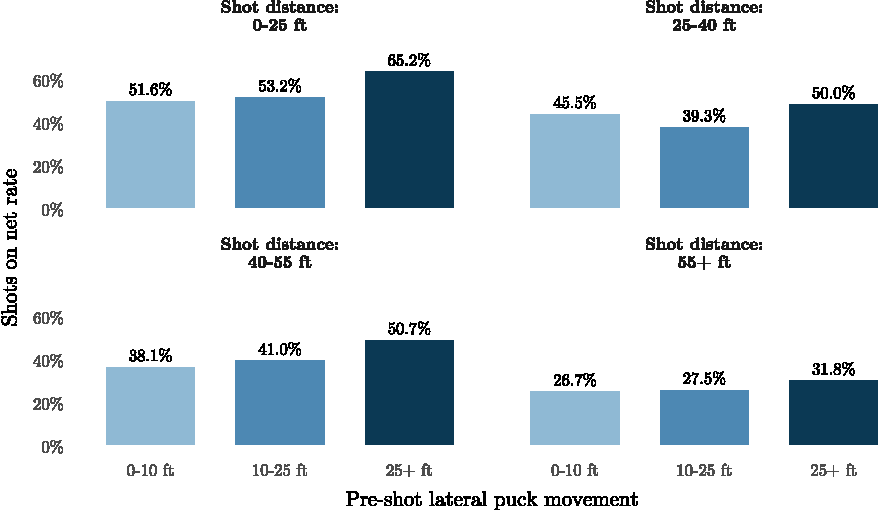
\includegraphics{Paper_files/figure-latex/fig-movement-1} 

}

\caption{Within every shot-distance band, the highest on-net rate comes from plays with at least 25 feet of lateral puck movement before the shot. Sample restricted to 5-on-5 shots preceded by a completed same-team play within five seconds (n = 655).}\label{fig:fig-movement}
\end{figure}

Figure 1 supports the thesis clearly. In every shot-distance band, the highest on-net rate comes from the largest movement group, the plays with at least 25 feet of lateral puck movement. Among shots from 0-25 feet, the on-net rate rises from 51.6\% after small 0-10 foot movement to 65.2\% after 25+ feet of movement. In the 25-40 foot band, it rises from 45.5\% to 50.0\%. In the 40-55 foot band, it rises from 38.1\% to 50.7\%. Even on long shots from 55+ feet, the biggest east-west plays still perform better, 26.7\% versus 31.8\%.

Just as importantly, this is not simply a closer-shot story. The biggest-movement group in my sample actually came from almost the same average shot distance as the smallest-movement group, 39.7 feet versus 39.1 feet. A logistic regression that controls for shot distance and shot width still finds a positive movement effect: each additional 10 feet of lateral pre-shot movement increased the odds that a shot ended on net by about 12.5\% and the 25+ foot group had about 1.53 times the on-net odds of the 0-10 foot group. This does not mean lateral movement explains every good chance, but it does mean the process leading into the shot carries independent information that a shot-only model can miss.

This result fits well with the published research. Yu et al.~argue that east-west pace changes shooting outcomes even when distance is held roughly constant; the Big Data Cup sample shows the same pattern in public competition data. Radke et al.~show why that should not be surprising: tracking data captures passing choices and receiver movement that ordinary shot logs compress away. The shared lesson is that offensive threat is not only about where a shot came from. It is also about whether the defense had time to get set.

\section{Conclusion}\label{conclusion}

The two sources support the same argument from different angles. Yu et al.~show at larger scale that pre-shot movement changes shot success beyond simple distance. Radke et al.~show that tracking can quantify passing options and moving targets that event summaries miss. My own analysis of the 2026 Big Data Cup sample extends that logic with a concrete public-data example: larger lateral puck movement before the shot is associated with better shot outcomes within every distance band I examined. That is enough evidence to defend a specific thesis: teams should not replace xG with tracking metrics, but they should add tracking-based pre-shot movement measures if they want a fuller picture of offensive creation.

A reasonable counterargument is that modern xG models already include some context, such as shot type, rush flags, or rebound indicators, and that my public sample is much smaller than a full NHL season. I do not think that is a major problem for the thesis, because I am arguing for supplementation rather than replacement. If pre-shot movement still matters after holding shot distance roughly constant, then teams lose information when they collapse everything back to the shot alone. The right response is broader validation, not a return to purely shot-based models.

The most useful future dataset would be frame-level optical or pose-tracking data that identifies goalie sightlines and defender stick positions at the moment of the pass and shot. That kind of data would let analysts distinguish two chances from the same x-y location when one is a clean one-timer into an open lane and the other is a screened point shot through traffic. In other words, it would help measure not only motion, but also visibility and access to the net.

\section{References}\label{references}

Big Data Cup. ``Big Data Cup 2026 Data Release.'\,' GitHub release. Accessed April 3, 2026. \url{https://github.com/bigdatacup/Big-Data-Cup-2026/releases/tag/Data}

Radke, David, Tim Brecht, and Daniel Radke. ``Identifying Completed Pass Types and Improving Passing Lane Models.'\,' Linköping Hockey Analytics Conference, 2022. \url{https://cs.uwaterloo.ca/~brecht/papers/passing-linhac-2022.pdf}

Yu, David, Christopher Boucher, Luke Bornn, and Mehrsan Javan. ``Playing Fast Not Loose: Evaluating team-level pace of play in ice hockey using spatio-temporal possession data.'\,' MIT Sloan Sports Analytics Conference Research Paper Competition, 2019. \url{https://www.lukebornn.com/papers/yu_sloan_2019.pdf}

\end{document}
